
\documentclass[11pt]{article}

\usepackage{common}
\usepackage{amsfonts}
\title{HW2: Tagging from Scratch}
\author{Alex Saich \\ asaich@seas.harvard.edu \and Colton Gyulay \\ cgyulay@seas.harvard.edu }
\begin{document}

\maketitle{}
\section{Introduction}

In the second problem set, our goal was to implement more advanced machine learning techniques to solve the problem of part-of-speech (POS) tagging. An emphasis on building end-to-end models with limited manual feature engineering played a large part in our motivation. In order to learn part-of-speech associations for individual words, we utilized word context windows around each target in order to leverage context for prediction. English linguist John Firth said it best: "You shall know a word by the company it keeps." Word context, along with a capitalization feature for each word in context, was used as input to our models.

We built three separate models for this task: a naive Bayes classifier, a logistic regression classifier, and a multilayer perceptron classifier (MLP), as seen in \cite{collobert2011natural}. The naive Bayes classifier learned a probability distribution by building a prior around which words and capitalization patters appeared in the context of certain tags. The logistic regression model used a sparse approach to learn context window and POS targets. The MLP, our most successful model, learned dense representations for each context word to make POS predictions. We also ran some MLP models with unsupervised, pre-trained word embeddings from \cite{pennington2014glove}, which we found yielded the best results.


\section{Problem Description}

\subsection{Dataset}

The primary dataset used was the Penn Treebank, which is comprised of around $50,000$ sentences, where each word has one of $45$ possible POS tags. For later models, we also used pre-trained word embeddings from \cite{collobert2011natural}, which were trained on 6B tokens from the Wikipedia 2014 and Gigaword 5 datasets. We also mapped each POS tag to a set $\mathcal{T}$ of size $\|\mathcal{T}\|$ (45). This informs the size $d_{out}$ in our models, as they are ultimately the classes that we want to predict.

The sentences were used to construct a unique vocabulary $\mcV$ of around 37,000 words, the size of our $d_{in}$. Words were treated as lower case only, though capitalization information about each word was saved as a separate context window. All numbers were mapped to the same token "NUMBER", while padding, mapped to a special "PADDING" token, was added to either side of the sentences to allow context windows for the beginning and ending words. Sentences were divided into context subsets of size $d_{win}$ = 5, where the assigned label was the tag for the central word. Although each input window was of size $1$ x $d_{win}$ since each word within the window is represented as an index value, the actual size of our input matrix $\boldX$ can be thought of as $d_{in}$ x $d_{win}$. The use of nn.LookupTable allows us to immediately convert to dense representation for our MLP.

Capitalization information was maintained by creating capitalization context windows for each word context window. Words could be sorted into one of $d_{cap} = 4$ categories: no capital letters, all capital letters, first letter capital, and any other letter(s) capital.

Finally, the pre-trained word vectors were used to boost our performance later during MLP training. Each word vector was of dimensionality $\reals^{1 x 50}$.

\subsection{Naive Bayes and Logistic Regression}

We used naive Bayes in a similar fashion as previously, although now two count matrices $\boldF_{word} \in \reals^{d_{in} x d_{win} x d_{out}}$, and $\boldF_{cap} \in \reals^{d_{cap} x d_{win} x d_{out}}$, were employed to record context probabilities. The probability for any word appearing in a class can be formalized as the following:
\begin{center}
$p(x, c|y_{\scriptscriptstyle i}) = \prod_{j=1}^{\|\mcV\|} p(x_{j}|y_{\scriptscriptstyle j})\prod_{k=1}^{d_{cap}}p(c_{k}|y_{\scriptscriptstyle l})$
\end{center}

Our naive Bayes model was optimized for the alpha coefficient $\alpha$, where values $0 < \alpha < 1$ (Lidstone smoothing) were compared with the value of 1 (Laplace smoothing).\\

For logistic regression, a similar model was built as the one used in Problem Set 1. The feature inputs were slightly more complex, as two input vectors $\boldx_{word} \in \mathbb{R}^{1 x d_{win}}$ and $\boldx_{cap} \in \mathbb{R}^{1 x d_{win}}$ were used to represent both the word and capitalization information in the window. In this representation, the size of the possible word input space is increased to $\|\mcV\|$ x $\|d_{win}\|$. The model learns to treat identical vocabulary words that are found in different positions as completely unrelated to one another, and a word in position -1 will have a completely different set of weights as the same word in another position.

This results in a much sparser weight vector than if position was ignored and words in different positions had the same weight, but maintains the position dimension of data that is important for learning POS associations. Depending on where specifically a word appears in the window can have vastly different implications the prediction. For instance, if a determinant appears in position -1 (directly before the central word), then it is highly likely that the central word is either an adjective or noun. If the same determinant appeared in position 1 then you can no longer make those same assumptions. This more complex model takes into account these stronger associations. Linear weight matrices $\boldW_{word} \in \mathbb{R}^{\|\mcV\| x \|\mathcal{T}\|}$, $\boldW_{cap} \in \mathbb{R}^{d_{cap} x \|\mathcal{T}\|}$ were used to transform the two inputs into vectors of size $1$ x $\|\mathcal{T}\|$, which were then combined and added to a bias term $\boldb \in \mathbb{R}^{\|\mathcal{T}\|}$. A $log$-$softmax$ layer was used to normalize the outputs from the regression.

\subsection{Multilayer Perceptron}

Finally we used an MLP which consists of multiple linear transformations with a non-linear function between these linear layers. The overall architecture of our model closely resembles that outlined in \cite{collobert2011natural}, with a similar word window input representation from our logistic regression. The same $\boldx_{word}$ and $\boldx_{cap}$ vectors were fed into weight vectors and then flattened along the second dimension $(d_{win})$ and combined. The result was an input vector that contained both word and capitalization information $\boldx \in \reals^{1 x d_{win} * (d_{embed} + d_{cap})$ = $\boldx \in \reals^{1 x d_{in_2}$.

The combined word and capitalization vectors are then fed into a classic linear layer, transformed by $\boldW_{0} \in \mathbb{R}^{d_{in_2} x d_{hid}}$, where $d_{hid}$ is the number of 'nodes' in the hidden layer of our perceptron model. The weight matrix $W_{0}$ has a corresponding bias term $b_{0} \in \mathbb{R}^{1 x d_{hid}}$. A nonlinearity is applied in the form of $tanh(x)$:
\begin{center}
$tanh(x) = \frac{exp(t) - exp(-t)}{exp(t) + exp(-t)}$
\end{center} 
The data is fed through another linear layer composed of weights $\boldW_{1} \in \mathbb{R}^{d_{hid} x d_{out}}$ and $\boldb_{1} \in \mathbb{R}^{d_{hid} x d_{out}}$ and finally a $log$-$softmax$ layer. The topology of the network is outlined more clearly in Figure 3.1, where the specific steps of each transformation are shown that lead to the eventual prediction output. A summary of notation can be seen in the table below.

  \begin{center}
    \begin{tabular}{@{}lll@{}}
      \toprule
      &\multicolumn{2}{c}{Notation} \\
      & Feature & Symbol\\
      \midrule
      & Vocabulary & $\mcV, d_{in}$ \\
      & Window Size & $d_{win}$ \\
      & Capitalization Options & $d_{cap}$ \\
      & Parts-of-Speech & $\mathcal{T}, d_{out}$ \\
      & Word Input Vector & $\boldx_{word}$\\
      & Cap. Input Vector & $\boldx_{cap}$\\
      & N.B. Smoothing Coefficient & $\alpha$ \\
      & MLP Learning Rate & $\eta$\\
      & MLP First Hidden Layer Size & $d_{hid}$\\
      & MLP Second Hidden Layer Size & $d_{hid_2}$ \\
      \bottomrule
    \end{tabular}
  \end{center}

\subsection{Multilayer Perceptron Variations}

\hspace{3ex}\textbf{Pre-Trained Word Embedding Vectors}

Rather than initializing our initial lookup table weights with randomized values, we utilized the pre-trained word embeddings from \cite{pennington2014glove}, which had made training dramatically faster.\\

\textbf{2-Layer MLP Model}

We ran another perceptron model with additional nonlinear and linear layers, so that two hidden layers of nodes processed input. After the input vector is run through our first $tanh(x)$ function, it is put through an additional weight matrix $W_{1} \in \reals^{d_{hid} x d_{hid_2}}$, where $d_{hid_2}$ is the size of the additional hidden layer dimension. The inputs are then run through another $tanh(x)$ function and then an eventual last weight matrix.\\

\section{Model and Algorithms}

A high level description of each model was given in the previous descrption, and here we will more formally present the topology of each of our models. The naive Bayes model essentially extracts word and capitalization co-occurrences for each output POS. After extracting this information from the dataset, predictions are made by multiplying a class prior by the product of each word and capitalization occurrence prior. The final predicted class is the entry with the maximum score from $log-softmax$. The Torch code for prediction is as follows:
\begin{verbatim}
function predict(word_windows, cap_windows)
  local pred = torch.IntTensor(word_windows:size(1))
  for i = 1, word_windows:size(1) do
    local word_window = word_windows[i]
    local cap_window = cap_windows[i]

    local p_y_hat = torch.zeros(nclasses)
    for y = 1, nclasses do
      p_y_hat[y] = p_y[y]

      -- Multiply p_y_hat by p(word at j|y) and p(cap at j|y)
      for j = 1, dwin do
        w = word_window[j]
        c = cap_window[j]

        p_y_hat[y] = p_y_hat[y] * word_alpha[y][j][w]
        p_y_hat[y] = p_y_hat[y] * cap_alpha[y][j][c]
      end
    end

    p_y_hat:div(p_y_hat:sum())
    val, prediction = torch.max(p_y_hat, 1)

    pred[i] = prediction
  end
  return pred
end
\end{verbatim}

In the implementation of both the logistic regression and MLP, we fed the word and capitalization windows through parallel tables, and then summed each table's output to create the full input to the rest of the layers. The Torch implementation of logistic regression was as follows:
\begin{verbatim}
nn.Sequential {
  [input -> (1) -> (2) -> (3) -> output]
  (1): nn.ParallelTable {
    input
      |`-> (1): nn.Sequential {
      |      [input -> (1) -> (2) -> output]
      |      (1): nn.LookupTable
      |      (2): nn.Sum
      |    }
      |`-> (2): nn.Sequential {
      |      [input -> (1) -> (2) -> output]
      |      (1): nn.LookupTable
      |      (2): nn.Sum
      |    }
       ... -> output
  }
  (2): nn.CAddTable
  (3): nn.LogSoftMax
}
\end{verbatim}

And the Torch implementation of the MLP was as follows:
\begin{verbatim}
nn.Sequential {
  [input -> (1) -> (2) -> (3) -> (4) -> (5) -> (6) -> output]
  (1): nn.ParallelTable {
    input
      |`-> (1): nn.Sequential {
      |      [input -> (1) -> (2) -> output]
      |      (1): nn.LookupTable
      |      (2): nn.Reshape(250)
      |    }
      |`-> (2): nn.Sequential {
      |      [input -> (1) -> (2) -> output]
      |      (1): nn.LookupTable
      |      (2): nn.Reshape(25)
      |    }
       ... -> output
  }
  (2): nn.JoinTable
  (3): nn.Linear(275 -> 300)
  (4): nn.HardTanh
  (5): nn.Linear(300 -> 45)
  (6): nn.LogSoftMax
}
\end{verbatim}

We've also included a graphic of the network's topology to illustrate the transformations present to execute POS predictions:
\begin{center}
    \includegraphics[width=12cm, height=8cm]{mlp.jpg}
\end{center}

Our vanilla MLP uses randomly initialized weights for the first lookup table $\boldW_{word}$, while our MLP+LM1 model uses pre-trained embeddings from \cite{pennington2014glove}. We also experimented with a two hidden layer model MLP2+LM1 which features an additional nonlinearity $tanh(x)$ and linear layer of size $d_{hid_2} = 200$.

\subsection{Training}
To train our logistic regression and MLP models we primarily used minibatch stochastic gradient descent with a minibatch size of 32. Training was done using the Torch library optim. Using optim we were able to achieve relatively fast training for each epoch. With $d_{hid} = 300$ and $\eta = 0.01$, our MLP achieved an average epoch training time of roughly 2 minutes. We also experimented with the gradient descent methods $adagrad$ and $rmsprop$, though neither produced better times or accuracy than standard minibatch SGD.

\section{Experiments}

As expected, the MLP performed best out of all models. The naive Bayes classifier performed strongly with dramatically less training time than either the logistic regression or MLP as it requires only one pass over the dataset. Given time, however, MLP model yield accuracy a few percentage points higher. Unfortunately, the performance of our linear regression model was subpar. The MLP+LM1 model using $d_{hid} = 300$ and an $\eta$ on an annealing schedule from 0.04 to 0.01 over 20 epochs achieved our best result, producing a validation accuracy of 96.53%.

\subsection{Naive Bayes}
The only hyperparameter we tuned for naive Bayes was the smooth coefficient $\alpha$, which we found to be optimal around $\alpha = 0.01$.

\begin{center}
    \includegraphics[width=12cm, length=10cm]{nb.png}\\
    \textit{Figure 1: Tuning hyperparamater $\alpha$ in naive Bayes classifier.}
\end{center}

\subsection{Logistic Regression}
The logistic regression model we built used unary features, treating each word as a different set of weights depending on its position in the context window. This dramatically increased vocabulary size as well as training time over the other models. Unfortunately, we were not able to replicate the performance of the naive Bayes or MLP models with logistic regression. A summary of its validation and training accuracy is seen in \textit{Figure 2}.

\begin{center}
    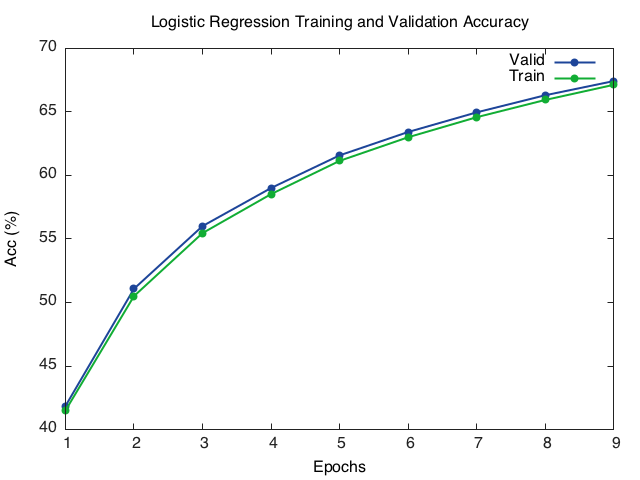
\includegraphics[width=12cm, length=10cm]{lracc.png}\\
    \textit{Figure 1: Logistic regression training and validation accuracy.}
\end{center}

\subsection{MLP}

Most of our experimentation was with the MLP model. We trained models with different learning rates, different hidden layer sizes, different numbers of hidden layers, and different embedding initializations. Surprisingly, increasing the number of hidden units and increasing the number of hidden layers produced marginal benefit, if any at all. Following the lead of \cite{collobert2011natural}, we initially trained with a learning rate of $\eta = 0.01$, but after tests found an annealing schedule ranging from $\eta = 0.04$ to $\eta = 0.01$ to yield the highest performance. A comparison of different learning rates can be seen in \textit{Figure 3}.

\begin{center}
    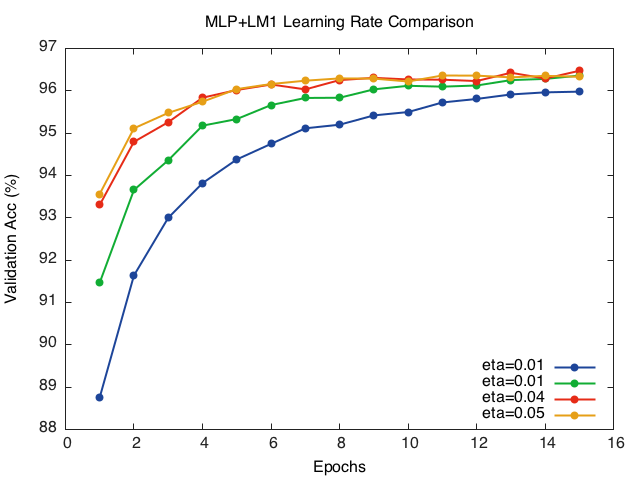
\includegraphics[width=12cm]{etacomparison.png}\\
    \textit{Figure 3: Comparing different learning rates for MLP+LM1.}
\end{center}

The pre-trained word embeddings made the most significant impact on our prediction performance, increasing validation accuracy over 15 epochs from 91.85 to 96.53. A comparison between random initialization and pre-trained embedding initialization is given in \textit{Figure 4}.

\begin{center}
    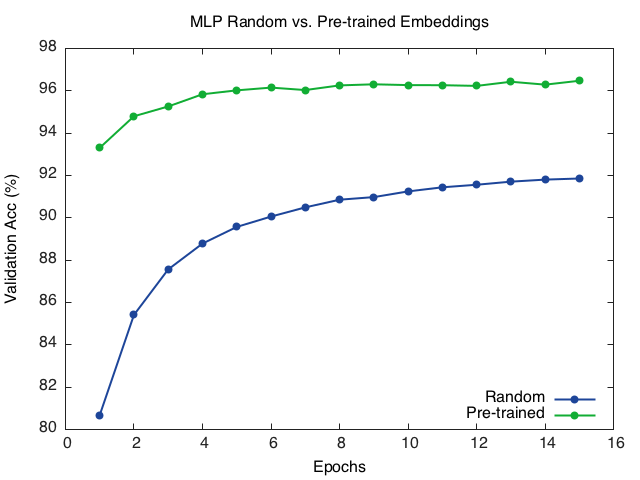
\includegraphics[width=12cm]{embeddings.png}\\
    \textit{Figure 4: Comparing MLP to MLP+LM1.}
\end{center}

There was a consistent difference of a couple percentage points between our validation and training accuracy. This is evidence of slight overfitting, which wasn't a huge negative as validation performance was still strong. MLP+LM1 loss divergence between training and validation can be seen in \textit{Figure 4}. \textit{Figure 5} shows this divergence for MLP2+LM1.

\begin{center}
    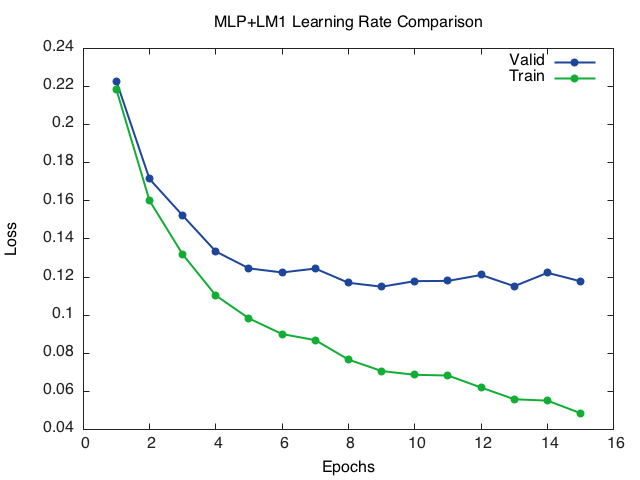
\includegraphics[width=12cm]{validvstrain.png}\\
    \textit{Figure 4: Comparing MLP+LM1 training and validation loss.}
\end{center}

\begin{center}
    \includegraphics[width=8cm, length=6cm]{2-layerMLP.png}
    \includegraphics[width=8cm, length=6cm]{2-layerloss.png}\\
    \textit{Figure 5: MLP2+LM1. Shown above is model performance over 15 epochs.}
\end{center}

\textit{Table 1} presents a final summary of our training and validation results across all models. Our best performing model was the one outlined by the \cite{collobert2011natural} paper, with hyperparameters and topology very closely mirroring those of the paper (pre-trained word embeddings of size 50 and $d_{hid} = 300$. Our adjustment of $\eta$ improved our own network's performance, though we were unable to reach their benchmark.

\begin{table}[h]
\centering
\begin{tabular}{llr}
 \toprule
 Model & Validation Acc (\%) & Training Acc (\%) \\
 \midrule
 \textsc{Naive Bayes} & 93.68 & 97.73 \\
 \textsc{Logistic Regression} & 67.42 & 67.13\\
 \textsc{MLP} & 91.85 & 94.35\\
 \textsc{MLP+LM1} & 96.53 & 98.37\\
 \textsc{MLP2+LM1} & 96.52 & 98.73\\
 \bottomrule
\end{tabular}
\caption{\label{tab:results} Accuracy results from our main tests.}
\end{table}

\section{Conclusion}

In conclusion, we were able to achieve strong results in the POS tagging task, though we couldn't exactly match the performance of the best model in \cite{collobert2011natural}. The hyperparamters specified in that paper were also very well tuned. Experiments we ran on increasing the number of hidden units and/or increasing the number of hidden layers did not yield noticeable gains in accuracy. Using a higher learning rate with an annealing schedule, however, did help us improve over training with a stable learning rate. With more time, we would've also liked to see better performance from the logistic regression model.

Our focus was on producing end-to-end models with minimal manual feature engineering. We could've pushed our accuracy higher, however, with providing features specifically for the prefixes or suffixes of words, and potentially the stem as well. Intuitively, the suffix at least can provide good indication of a word's part-of-speech.

Using the unsupervised, pre-trained word embeddings from \cite{pennington2014glove} provided a boost in performance as well as a significant boost in accuracy in early epochs. Allowing the gradients to propagate to these weights during training fine-tuned them to the task, even though they were initialized to solve a slightly different task (word prediction given context, rather than POS prediction).

One final improvement might come in further combating overfitting. We consistently saw our models score a couple percentage points higher on training accuracy over validation accuracy. We ran some experiments with dropout layers and ReLU nonlinearities, but were unable to replicate the results we saw with the $tanh(x)$ activation.

\bibliographystyle{apalike}
\bibliography{writeup}

\end{document}
